\PassOptionsToPackage{unicode=true}{hyperref} % options for packages loaded elsewhere
\PassOptionsToPackage{hyphens}{url}
%
\documentclass[ignorenonframetext,]{beamer}
\usepackage{pgfpages}
\setbeamertemplate{caption}[numbered]
\setbeamertemplate{caption label separator}{: }
\setbeamercolor{caption name}{fg=normal text.fg}
\beamertemplatenavigationsymbolsempty
% Prevent slide breaks in the middle of a paragraph:
\widowpenalties 1 10000
\raggedbottom
\setbeamertemplate{part page}{
\centering
\begin{beamercolorbox}[sep=16pt,center]{part title}
  \usebeamerfont{part title}\insertpart\par
\end{beamercolorbox}
}
\setbeamertemplate{section page}{
\centering
\begin{beamercolorbox}[sep=12pt,center]{part title}
  \usebeamerfont{section title}\insertsection\par
\end{beamercolorbox}
}
\setbeamertemplate{subsection page}{
\centering
\begin{beamercolorbox}[sep=8pt,center]{part title}
  \usebeamerfont{subsection title}\insertsubsection\par
\end{beamercolorbox}
}
\AtBeginPart{
  \frame{\partpage}
}
\AtBeginSection{
  \ifbibliography
  \else
    \frame{\sectionpage}
  \fi
}
\AtBeginSubsection{
  \frame{\subsectionpage}
}
\usepackage{lmodern}
\usepackage{amssymb,amsmath}
\usepackage{ifxetex,ifluatex}
\usepackage{fixltx2e} % provides \textsubscript
\ifnum 0\ifxetex 1\fi\ifluatex 1\fi=0 % if pdftex
  \usepackage[T1]{fontenc}
  \usepackage[utf8]{inputenc}
  \usepackage{textcomp} % provides euro and other symbols
\else % if luatex or xelatex
  \usepackage{unicode-math}
  \defaultfontfeatures{Ligatures=TeX,Scale=MatchLowercase}
\fi
\usetheme[]{Hannover}
\usecolortheme{dove}
\usefonttheme{structurebold}
% use upquote if available, for straight quotes in verbatim environments
\IfFileExists{upquote.sty}{\usepackage{upquote}}{}
% use microtype if available
\IfFileExists{microtype.sty}{%
\usepackage[]{microtype}
\UseMicrotypeSet[protrusion]{basicmath} % disable protrusion for tt fonts
}{}
\IfFileExists{parskip.sty}{%
\usepackage{parskip}
}{% else
\setlength{\parindent}{0pt}
\setlength{\parskip}{6pt plus 2pt minus 1pt}
}
\usepackage{hyperref}
\hypersetup{
            pdftitle={Session 4: loglinear regression part 1},
            pdfauthor={Levi Waldron},
            pdfborder={0 0 0},
            breaklinks=true}
\urlstyle{same}  % don't use monospace font for urls
\newif\ifbibliography
\usepackage{graphicx,grffile}
\makeatletter
\def\maxwidth{\ifdim\Gin@nat@width>\linewidth\linewidth\else\Gin@nat@width\fi}
\def\maxheight{\ifdim\Gin@nat@height>\textheight\textheight\else\Gin@nat@height\fi}
\makeatother
% Scale images if necessary, so that they will not overflow the page
% margins by default, and it is still possible to overwrite the defaults
% using explicit options in \includegraphics[width, height, ...]{}
\setkeys{Gin}{width=\maxwidth,height=\maxheight,keepaspectratio}
\setlength{\emergencystretch}{3em}  % prevent overfull lines
\providecommand{\tightlist}{%
  \setlength{\itemsep}{0pt}\setlength{\parskip}{0pt}}
\setcounter{secnumdepth}{0}

% set default figure placement to htbp
\makeatletter
\def\fps@figure{htbp}
\makeatother


\title{Session 4: loglinear regression part 1}
\author{Levi Waldron}
\providecommand{\institute}[1]{}
\institute{CUNY SPH Biostatistics 2}
\date{}

\begin{document}
\frame{\titlepage}

\hypertarget{learning-objectives-and-outline}{%
\section{Learning objectives and
outline}\label{learning-objectives-and-outline}}

\begin{frame}{Learning objectives}
\protect\hypertarget{learning-objectives}{}

\begin{enumerate}
\tightlist
\item
  Define log-linear models in GLM framework
\item
  Identify situations that motivate use of log-linear models
\item
  Define the Poisson distribution and the log-linear Poisson GLM
\item
  Identify applications and properties of the Poisson distribution
\item
  Define multi-collinearity
\end{enumerate}

\end{frame}

\begin{frame}{Outline}
\protect\hypertarget{outline}{}

\begin{enumerate}
\tightlist
\item
  Brief review of GLMs
\item
  Motivating example for log-linear models
\item
  Poisson log-linear GLM
\item
  Note on collinearity
\end{enumerate}

Reading: Vittinghoff textbook chapter 8.1-8.3

\end{frame}

\hypertarget{review}{%
\section{Review}\label{review}}

\begin{frame}{Components of GLM}
\protect\hypertarget{components-of-glm}{}

\begin{itemize}
\tightlist
\item
  \textbf{Random component} specifies the conditional distribution for
  the response variable - it doesn't have to be normal but can be any
  distribution that belongs to the ``exponential'' family of
  distributions
\item
  \textbf{Systematic component} specifies linear function of predictors
  (linear predictor)
\item
  \textbf{Link} {[}denoted by g(.){]} specifies the relationship between
  the expected value of the random component and the systematic
  component, can be linear or nonlinear
\end{itemize}

\end{frame}

\begin{frame}{Linear Regression as GLM}
\protect\hypertarget{linear-regression-as-glm}{}

\begin{itemize}
\item
  \textbf{The model}:
  \(y_i = E[y|x] + \epsilon_i = \beta_0 + \beta_1 x_{1i} + \beta_2 x_{2i} + ... + \beta_p x_{pi} + \epsilon_i\)
\item
  \textbf{Random component} of \(y_i\) is normally distributed:
  \(\epsilon_i \stackrel{iid}{\sim} N(0, \sigma_\epsilon^2)\)
\item
  \textbf{Systematic component} (linear predictor):
  \(\beta_0 + \beta_1 x_{1i} + \beta_2 x_{2i} + ... + \beta_p x_{pi}\)
\item
  \textbf{Link function} here is the \emph{identity link}:
  \(g(E(y | x)) = E(y | x)\). We are modeling the mean directly, no
  transformation.
\end{itemize}

\end{frame}

\begin{frame}{Logistic Regression as GLM}
\protect\hypertarget{logistic-regression-as-glm}{}

\begin{itemize}
\item
  \textbf{The model}: \[
  Logit(P(x)) = log \left( \frac{P(x)}{1-P(x)} \right) = \beta_0 + \beta_1 x_{1i} + \beta_2 x_{2i} + ... + \beta_p x_{pi}
  \]
\item
  \textbf{Random component}: \(y_i\) follows a Binomial distribution
  (outcome is a binary variable)
\item
  \textbf{Systematic component}: linear predictor \[
  \beta_0 + \beta_1 x_{1i} + \beta_2 x_{2i} + ... + \beta_p x_{pi}
  \]
\item
  \textbf{Link function}: \emph{logit} (Converts Prob -\textgreater{}
  log-odds) \[
  g(P(x)) = logit(P(x)) = log\left( \frac{P(x)}{1-P(x)} \right)
  \] \[
  P(x) = g^{-1}\left( \beta_0 + \beta_1 x_{1i} + \beta_2 x_{2i} + ... + \beta_p x_{pi}
   \right)
  \]
\end{itemize}

\end{frame}

\begin{frame}{Additive vs.~Multiplicative models}
\protect\hypertarget{additive-vs.multiplicative-models}{}

\begin{itemize}
\tightlist
\item
  Linear regression is an \emph{additive} model

  \begin{itemize}
  \tightlist
  \item
    \emph{e.g.} for two binary variables \(\beta_1 = 1.5\),
    \(\beta_2 = 1.5\).
  \item
    If \(x_1=1\) and \(x_2=1\), this adds 3.0 to \(E(y|x)\)
  \end{itemize}
\item
  Logistic regression is a \emph{multiplicative} model

  \begin{itemize}
  \tightlist
  \item
    If \(x_1=1\) and \(x_2=1\), this adds 3.0 to \(log(\frac{P}{1-P})\)
  \item
    Odds-ratio \(\frac{P}{1-P}\) increases 20-fold: \(exp(1.5+1.5)\) or
    \(exp(1.5) * exp(1.5)\)
  \end{itemize}
\end{itemize}

\end{frame}

\hypertarget{motivating-example-for-log-linear-models}{%
\section{Motivating example for log-linear
models}\label{motivating-example-for-log-linear-models}}

\begin{frame}{Effectiveness of a depression case-management program}
\protect\hypertarget{effectiveness-of-a-depression-case-management-program}{}

\begin{itemize}
\tightlist
\item
  Research question: can a new treatment reduce the number of needed
  visits to the emergency room, compared to standard care?
\item
  \emph{outcome}: \# of emergency room visits for each patient in the
  year following initial treatment
\item
  \emph{predictors}:

  \begin{itemize}
  \tightlist
  \item
    \emph{race} (white or nonwhite)
  \item
    \emph{treatment} (treated or control)
  \item
    \emph{amount of alcohol consumption} (numerical measure)
  \item
    \emph{drug use} (numerical measure)
  \end{itemize}
\end{itemize}

\end{frame}

\begin{frame}{Statistical issues}
\protect\hypertarget{statistical-issues}{}

\begin{enumerate}
\tightlist
\item
  about 1/3 of observations are exactly 0 (did not return to the
  emergency room within the year)
\item
  highly nonnormal and cannot be transformed to be approximately normal
\item
  even \(log(y_i + 1)\) transformation will have a ``lump'' at zero +
  over 1/2 the transformed data would have values of 0 or \(log(2)\)
\item
  a linear regression model would give negative predictions for some
  covariate combinations
\item
  some subjects die or cannot be followed up on for a whole year
\end{enumerate}

\end{frame}

\begin{frame}{Towards a reasonable model}
\protect\hypertarget{towards-a-reasonable-model}{}

\begin{itemize}
\tightlist
\item
  A \emph{multiplicative} model will allow us to make inference on
  \emph{ratios} of mean emergency room usage
\item
  Modeling \(log\) of the \emph{mean} emergency usage ensures positive
  means, and does not suffer from \(log(0)\) problem
\item
  Random component of GLM, or residuals (was
  \(\epsilon_i \stackrel{iid}{\sim} N(0, \sigma_\epsilon^2)\) for linear
  regression) may still not be normal, but we can choose from other
  distributions
\end{itemize}

\end{frame}

\begin{frame}{Proposed model without time}
\protect\hypertarget{proposed-model-without-time}{}

\[
log(E[Y_i]) = \beta_0 + \beta_1 \textrm{RACE}_i + \beta_2 \textrm{TRT}_i + \beta_3 \textrm{ALCH}_i + \beta_4 \textrm{DRUG}_i
\] Or equivalently: \[
E[Y_i] = exp \left( \beta_0 + \beta_1 \textrm{RACE}_i + \beta_2 \textrm{TRT}_i + \beta_3 \textrm{ALCH}_i + \beta_4 \textrm{DRUG}_i \right)
\] where \(E[Y_i]\) is the expected number of emergency room visits for
patient \emph{i}.

\begin{itemize}
\tightlist
\item
  Important note: Modeling \(log(E[Y_i])\) is \emph{not} equivalent to
  modeling \(E(log(Y_i))\)
\end{itemize}

\end{frame}

\begin{frame}{Accounting for follow-up time}
\protect\hypertarget{accounting-for-follow-up-time}{}

Instead, model mean count per unit time: \[
\begin{aligned}
log(E[Y_i]/t_i) = \beta_0 + \beta_1 \textrm{RACE}_i + \beta_2 \textrm{TRT}_i + 
\beta_3 \textrm{ALCH}_i + \nonumber \\ \beta_4 \textrm{DRUG}_i
\end{aligned}
\]

Or equivalently: \[
\begin{aligned}
log(E[Y_i]) = \beta_0 + \beta_1 \textrm{RACE}_i + \beta_2 \textrm{TRT}_i + 
\beta_3 \textrm{ALCH}_i + \nonumber \\ \beta_4 \textrm{DRUG}_i + log(t_i)
\end{aligned}
\]

\begin{itemize}
\tightlist
\item
  \(log(t_i)\) is not a covariate, it is called an \emph{offset}
\end{itemize}

\end{frame}

\begin{frame}{The Poisson distribution}
\protect\hypertarget{the-poisson-distribution}{}

\begin{itemize}
\tightlist
\item
  Count data are often modeled as Poisson distributed:

  \begin{itemize}
  \tightlist
  \item
    mean \(\lambda\) is greater than 0
  \item
    variance is also \(\lambda\)
  \item
    Probability density
    \(P(k, \lambda) = \frac{\lambda^k}{k!} e^{-\lambda}\)
  \end{itemize}
\end{itemize}

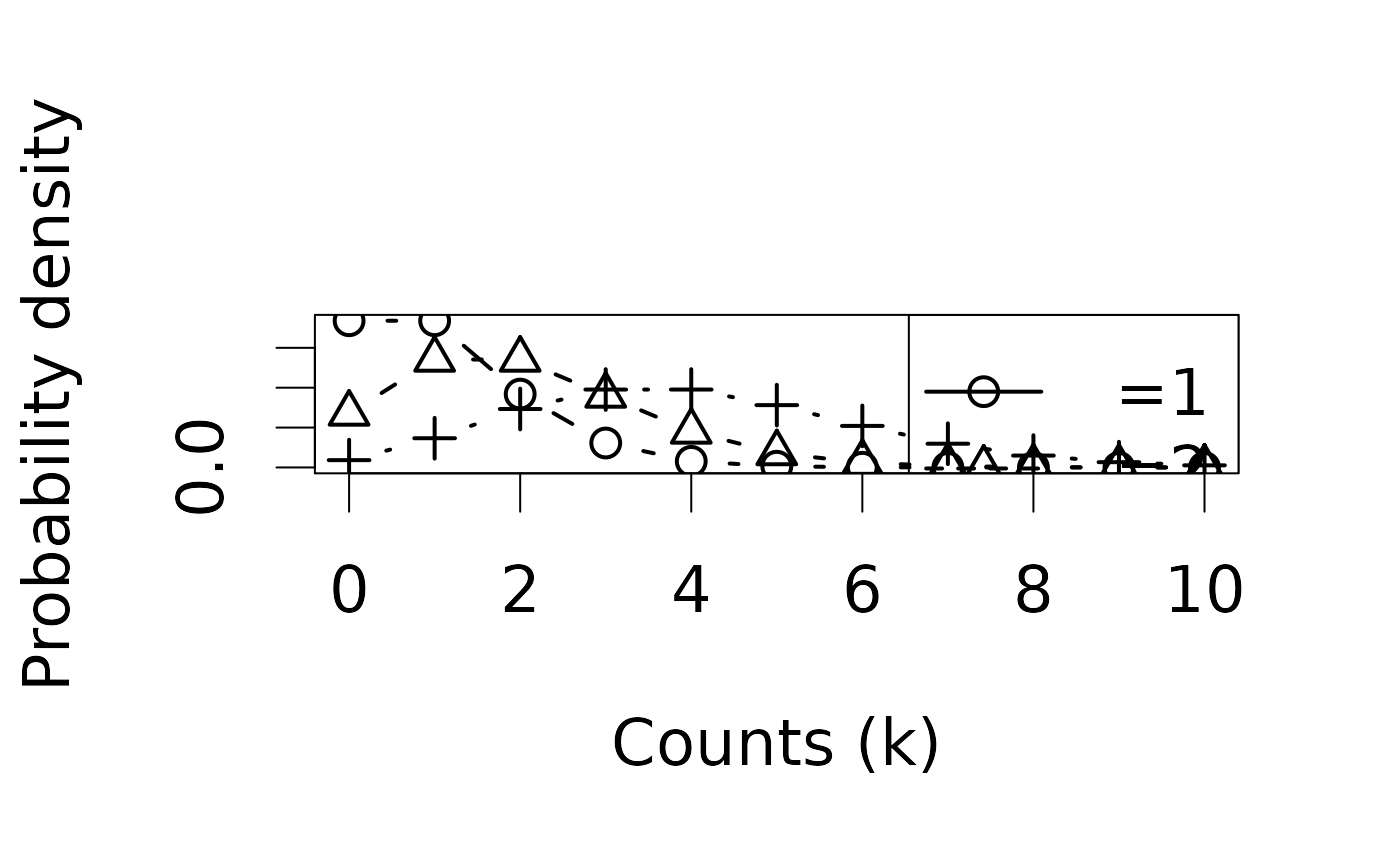
\includegraphics{../docs/articles/session_lecture_files/figure-beamer/unnamed-chunk-1-1.pdf}

\end{frame}

\begin{frame}{When the Poisson distribution works}
\protect\hypertarget{when-the-poisson-distribution-works}{}

\begin{itemize}
\tightlist
\item
  Individual events are low-probability (small p), but many
  opportunities (large n)

  \begin{itemize}
  \tightlist
  \item
    e.g. \# 911 calls per day
  \item
    e.g. \# emergency room visits
  \end{itemize}
\item
  Approximates the binomial distribution when n is large and p is small

  \begin{itemize}
  \tightlist
  \item
    e.g. \(n > 20\), \(np < 5\) or \(n(1-p) < 5\)
  \end{itemize}
\item
  When mean of residuals is approx. equal to variance
\end{itemize}

\end{frame}

\begin{frame}{GLM with log-linear link and Poisson error model}
\protect\hypertarget{glm-with-log-linear-link-and-poisson-error-model}{}

\begin{itemize}
\tightlist
\item
  Model the number of counts per unit time as Poisson-distributed + so
  the expected number of counts per time is \(\lambda_i\)
\end{itemize}

\(E[Y_i]/t_i = \lambda_i\) \newline \(log(E[Y_i]/t_i) = log(\lambda_i)\)
\newline \(log(E[Y_i]) = log(\lambda_i) + log(t_i)\) \newline

Recalling the log-linear model systematic component: \[
\begin{aligned}
log(E[Y_i]) = \beta_0 + \beta_1 \textrm{RACE}_i + \beta_2 \textrm{TRT}_i + 
\beta_3 \textrm{ALCH}_i + \nonumber \\ \beta_4 \textrm{DRUG}_i + log(t_i)
\end{aligned}
\]

\end{frame}

\begin{frame}{GLM with log-linear link and Poisson error model (cont'd)}
\protect\hypertarget{glm-with-log-linear-link-and-poisson-error-model-contd}{}

Then the systematic part of the GLM is: \[
log(\lambda_i) = \beta_0 + \beta_1 \textrm{RACE}_i + \beta_2 \textrm{TRT}_i + \beta_3 \textrm{ALCH}_i + \beta_4 \textrm{DRUG}_i
\] Or alternatively: \[
\lambda_i = exp \left( \beta_0 + \beta_1 \textrm{RACE}_i + \beta_2 \textrm{TRT}_i + \beta_3 \textrm{ALCH}_i + \beta_4 \textrm{DRUG}_i \right)
\]

\end{frame}

\begin{frame}{Interpretation of coefficients}
\protect\hypertarget{interpretation-of-coefficients}{}

\begin{itemize}
\tightlist
\item
  Suppose that \(\hat \beta_1 = -0.5\) in the fitted model, where
  \(\textrm{RACE}_i=0\) for white and \(\textrm{RACE}_i=1\) for
  non-white.
\item
  The mean rate of emergency room visits per unit time for white
  relative to non-white, all else held equal, is estimated to be:
\end{itemize}

\[
\frac{exp \left( \beta_0 + 0 + \beta_2 \textrm{TRT}_i + \beta_3 \textrm{ALCH}_i + \beta_4 \textrm{DRUG}_i \right)}{exp \left( \beta_0 - 0.5 + \beta_2 \textrm{TRT}_i + \beta_3 \textrm{ALCH}_i + \beta_4 \textrm{DRUG}_i \right)}
\] \[
= \frac{e^{\beta_0} e^0 e^{\beta_2 \textrm{TRT}_i} e^{\beta_3 \textrm{ALCH}_i} e^{\beta_4 \textrm{DRUG}_i}}
{e^{\beta_0} e^{-0.5} e^{\beta_2 \textrm{TRT}_i} e^{\beta_3 \textrm{ALCH}_i} e^{\beta_4 \textrm{DRUG}_i}}
\] \[
= \frac{e^0}{e^{-0.5}}
\] \[
= e^{0.5} \approxeq 1.65
\]

\end{frame}

\begin{frame}{Interpretation of coefficients (cont'd)}
\protect\hypertarget{interpretation-of-coefficients-contd}{}

\begin{itemize}
\tightlist
\item
  If \(\hat \beta_1=-0.5\) with whites as the reference group: - after
  adjustment for treatment group, alcohol and drug usage, whites tend to
  use the emergency room at a rate 1.65 times higher than non-whites. -
  equivalently, the average rate of usage for whites is 65\% higher than
  that for non-whites
\item
  Multiplicative rules apply for other coefficients as well, because
  they are exponentiated to estimate the mean rate.
\end{itemize}

\end{frame}

\hypertarget{multicollinearity}{%
\section{Multicollinearity}\label{multicollinearity}}

\begin{frame}{Note on Multicollinearity}
\protect\hypertarget{note-on-multicollinearity}{}

\begin{enumerate}
\tightlist
\item
  \emph{Multicollinearity} exists when two or more of the independent
  variables in regression are moderately or highly correlated.
\item
  Multicollinearity implies near-linear relationship among the
  predictors
\item
  The presence of near-linear dependence dramatically impacts the
  ability to estimate regression coefficients
\item
  High multicollinearity results in larger standard errors for
  regression coefficients

  \begin{itemize}
  \tightlist
  \item
    estimates of such regression coefficients will tend to be less
    stable over repeated sampling
  \end{itemize}
\end{enumerate}

\end{frame}

\hypertarget{conclusions}{%
\section{Conclusions}\label{conclusions}}

\begin{frame}{Conclusions}
\protect\hypertarget{conclusions-1}{}

\begin{enumerate}
\tightlist
\item
  Log-linear models are appropriate for non-negative, skewed count data

  \begin{itemize}
  \tightlist
  \item
    probability of each event is low
  \end{itemize}
\item
  The coefficients of log-linear models are \emph{multiplicative}
\item
  An \emph{offset} term can account for varying follow-up time or
  otherwise varying opportunity to be counted
\item
  Poisson distribution is limit of binomial distribution with high
  number of trials, low probability
\item
  Inference from log-linear models is sensitive to the choice of error
  model (assumption on the distribution of residuals)
\item
  We will cover other options next week for when the Poisson error model
  doesn't fit:

  \begin{itemize}
  \tightlist
  \item
    Variance proportional to mean, instead of equal
  \item
    Negative Binomial
  \item
    Zero Inflation
  \end{itemize}
\end{enumerate}

\end{frame}

\end{document}
